%Semantics of state charts
\section{\plcchart}
\label{sec:statechartsem}

The language used for our project was purposely modelled after \emphasize{UML2 State Machine Diagram}\cite{UML2}. As discussed in section \ref{sec:overviewstatechart} UML2 is similar to state machine with extensions added on to describe behaviours in states. The motivation in using \emphasize{UML2 State Machine Diagram}\cite{UML2} as a basis for \emphasize{\plcchart} consists of three primary details: First \emphasize{UML2 State Machine Diagram}\cite{UML2} is quite well known and popular, this improves the potential acceptance of our tool. Secondly \emphasize{UML2 State Machine Diagram}\cite{UML2} state machine syntax is more concrete than the other forms of state machines, giving a strong basis to construct our language around. Finally \emphasize{UML2 State Machine Diagram}\cite{UML2} has the concept of internal activity or internal execution necessary for modelling the behaviour of an actual useful program.

The model of \plcchart $\:$ is expressed mathematically as follows:

\begin{definition}
	\plcchart
	
\begin{itemize}
	\item \textbf{$Q$:} Set of modes.
	\item \textbf{$V$:} The state space $V = \langle V_0,V_1,V_2,..,V_n \rangle \: where \: V_{i}\in \lbrace \mathbb{Z}_{128}, \mathbb{Z}, \mathbb{B}, \mathbb{R} \rbrace$
	\item $\mathbf{v}_{init}$: vector of initial values $\mathbf{v}_{init}$: $\langle v_0,..,v_n \rangle \: where \: (v_i \in V_i)$
	\item \textbf{$G$:} Set of guard conditions. $V \rightarrow \mathbb{B}$
	\item \textbf{$A$:} Set of assignments. $V \times Q \rightarrow V$
	\item \textbf{$\tau$:} Set of transitions. $G \times Q \rightarrow Q$
	\item \textbf{$q_0$:} The initial starting mode.
\end{itemize}
\end{definition}

Many states in the system can belong to the same mode. A state space in our system is used for to model variables. All variables in \emphasize{\plcchart} are typed. The Initial value in the system is given by a vector of elements that come from the state spaces $V$.  Guard conditions are mappings from states spaces to boolean values.

Assignments in our system take the form $V \times Q \rightarrow V$. Suppose we the state $\langle 1,2 \rangle$ meaning $v_1 = 1, v_2 = 2$ suppose we are in mode $5$ an assignment $v1 := v2, v_2 := 0$ can be described by: $( \langle 1,2 \rangle,5) \rightarrow ( \langle 2,0 \rangle )$. Assignments to variables are always represented by changes to the state.

\begin{figure}[htp]
    \centering
    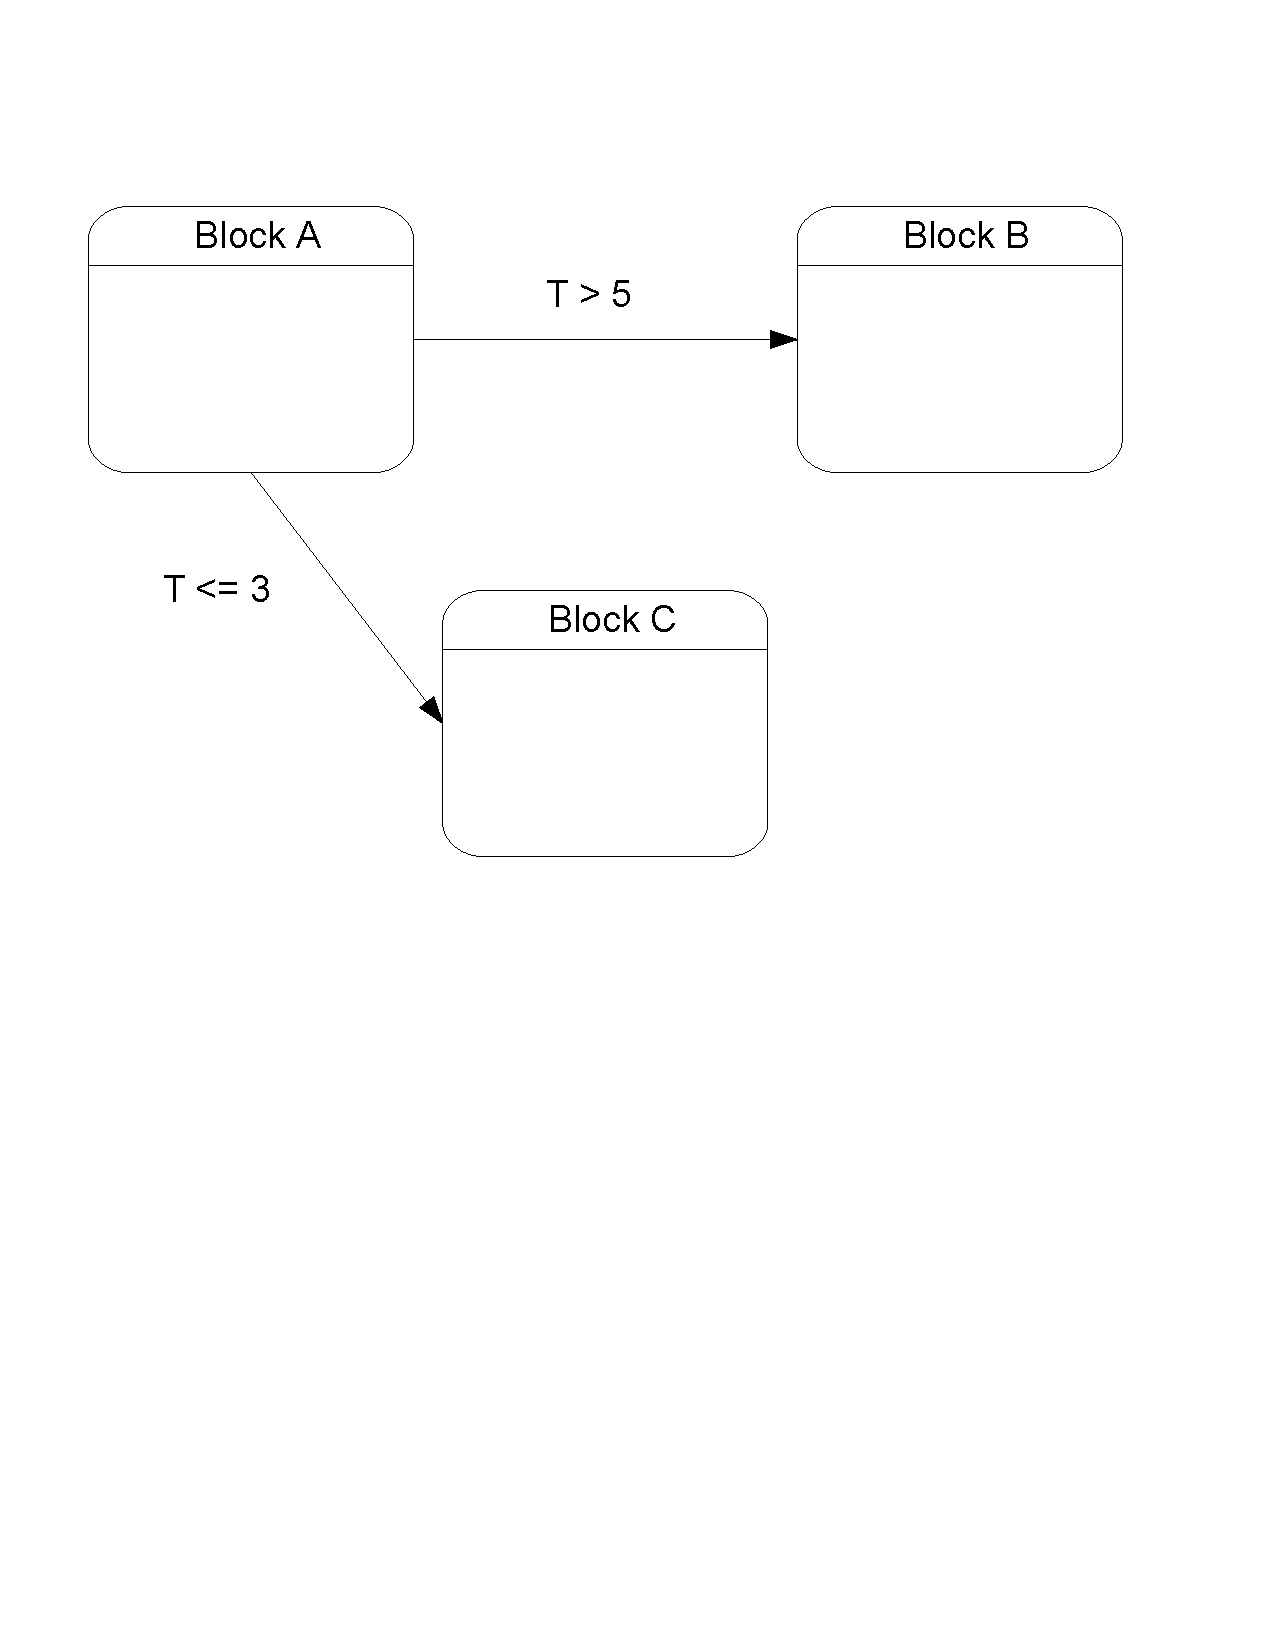
\includegraphics[trim= 10mm 130mm 20mm 10mm, clip, width=\imgmedphoto]{./images/state_transition.pdf}
    \caption{Example of Basic Transitions}
    \label{fig:state_transition_cor}
\end{figure}

\begin{figure}[htp]
    \centering
    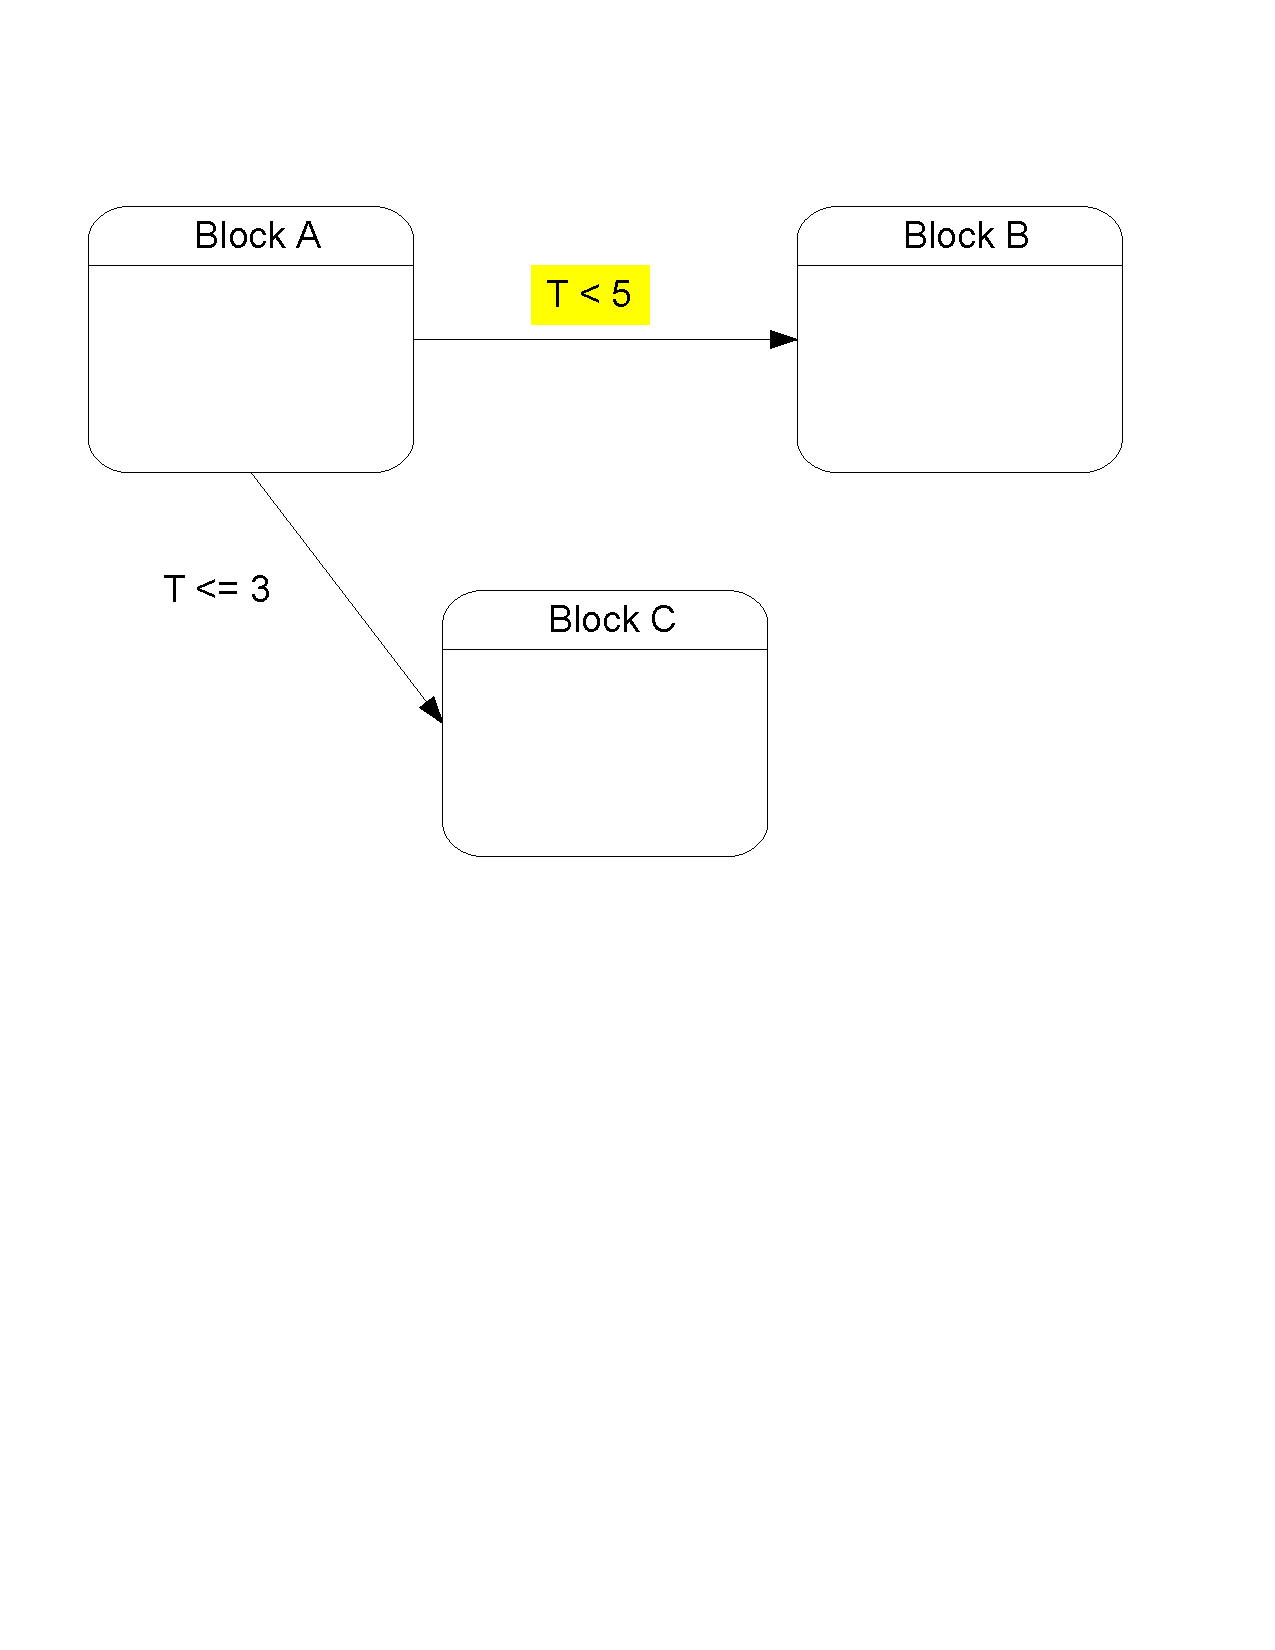
\includegraphics[trim= 10mm 130mm 20mm 10mm, clip, width=\imgmedphoto]{./images/state_transition_bad.pdf}
    \caption{Incorrect Transitions}
    \label{fig:state_transition_bad}
\end{figure}

Transitions in our system must start from an block object and must terminate at another block. Since \emphasize{\plcchart} does not support non-deterministic execution, transition conditions must be mutually exclusive to be valid. All edges departing a block must have ${\nexists{\tau} \forall{g \in G} \: \forall{q_1, q_2, q_3\in Q}} {({\tau(g,q_1) \rightarrow q_2} \wedge {\tau(g,q_1) \rightarrow q_3} \wedge {q_2 \neq q_3})}$. In Figure \ref{fig:state_transition_cor} we see three possible outcomes ($T<=3$,``Block A'') $\rightarrow$ ``Block C'',  \\
($T>5$,``Block A'') $\rightarrow$ ``Block B'', and for $3 < T <= 5$ we stay in ``Block A'' since there is no transition to take us out. An incorrect usage of transitions is shown in Figure \ref{fig:state_transition_bad}. Values of $T <= 3$ will cause both guard conditions to become true, violating our requirement for mutual exclsion. \emphasize{\plcchart} considers the outcome of mutliple possible transitions as undefined and is invalid in the language.
